\chapter{Appendices}
\section{Appendix A: Tools Used}

\begin{figure}[H]
\center
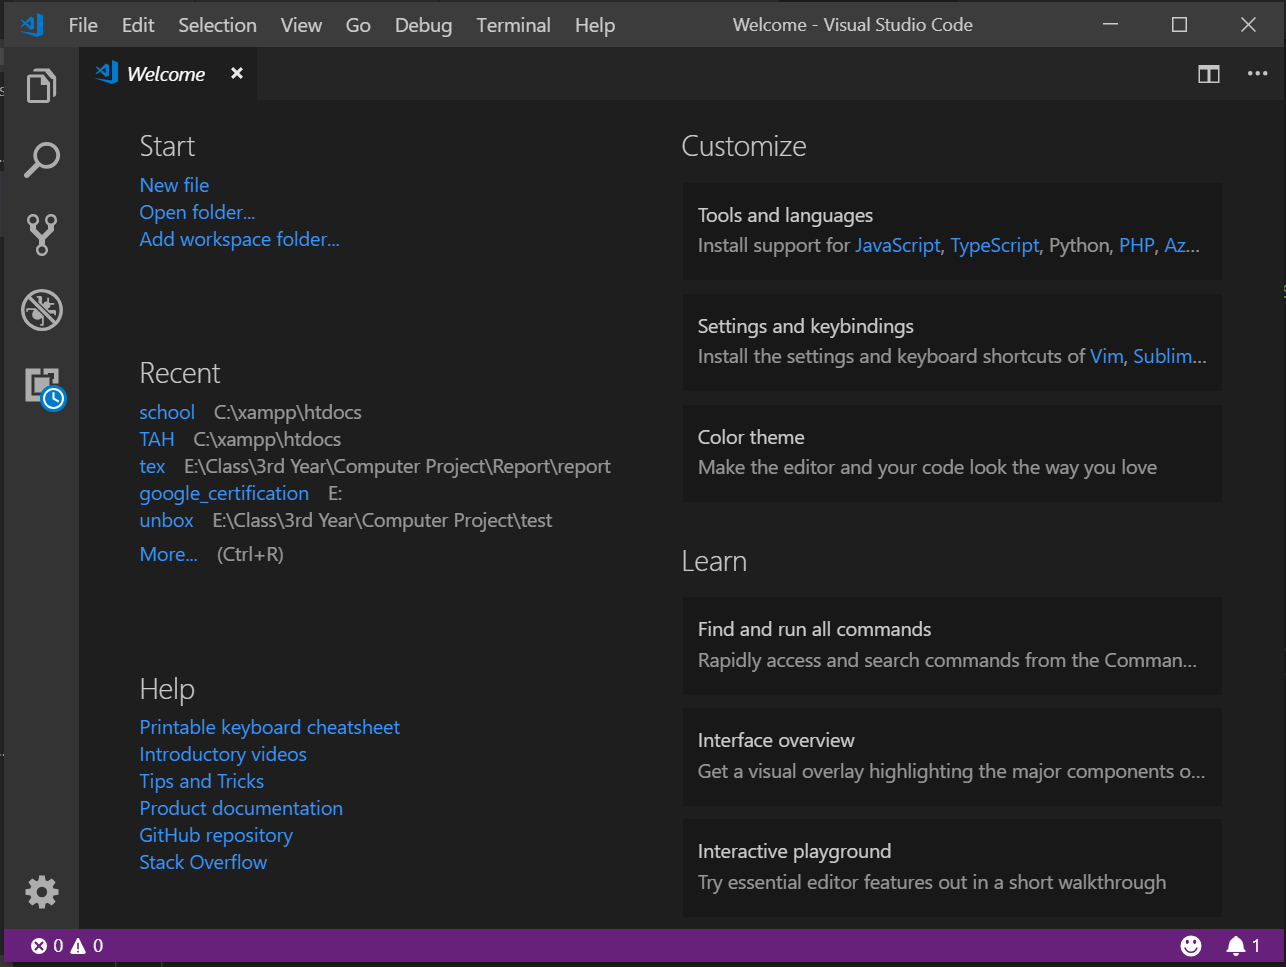
\includegraphics[scale=0.4]{images/vscode.png}
\caption{Visual Studio Code, the text editor used to write code for the system.}
\end{figure}

\begin{figure}[H]
\center
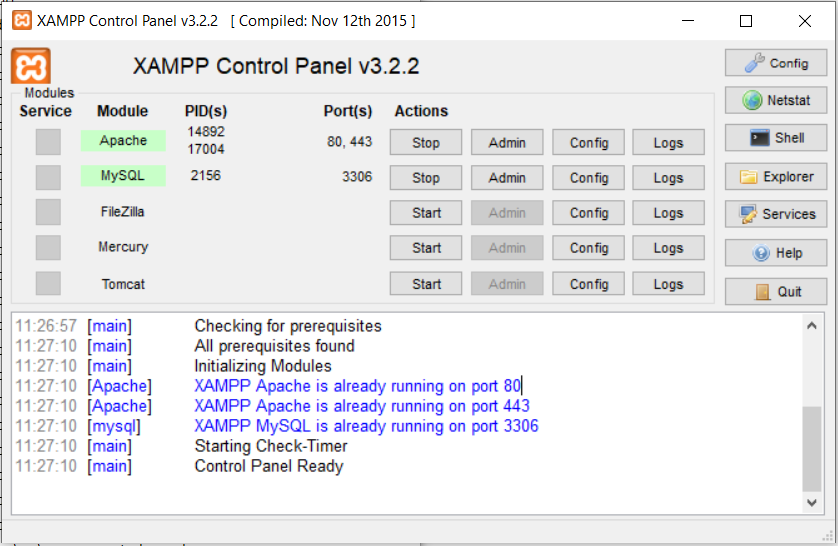
\includegraphics[scale=0.5]{images/XAMPP_cp.png}
\caption{The control panel for the XAMPP local development environment.}
\end{figure}

\begin{figure}[H]
\center
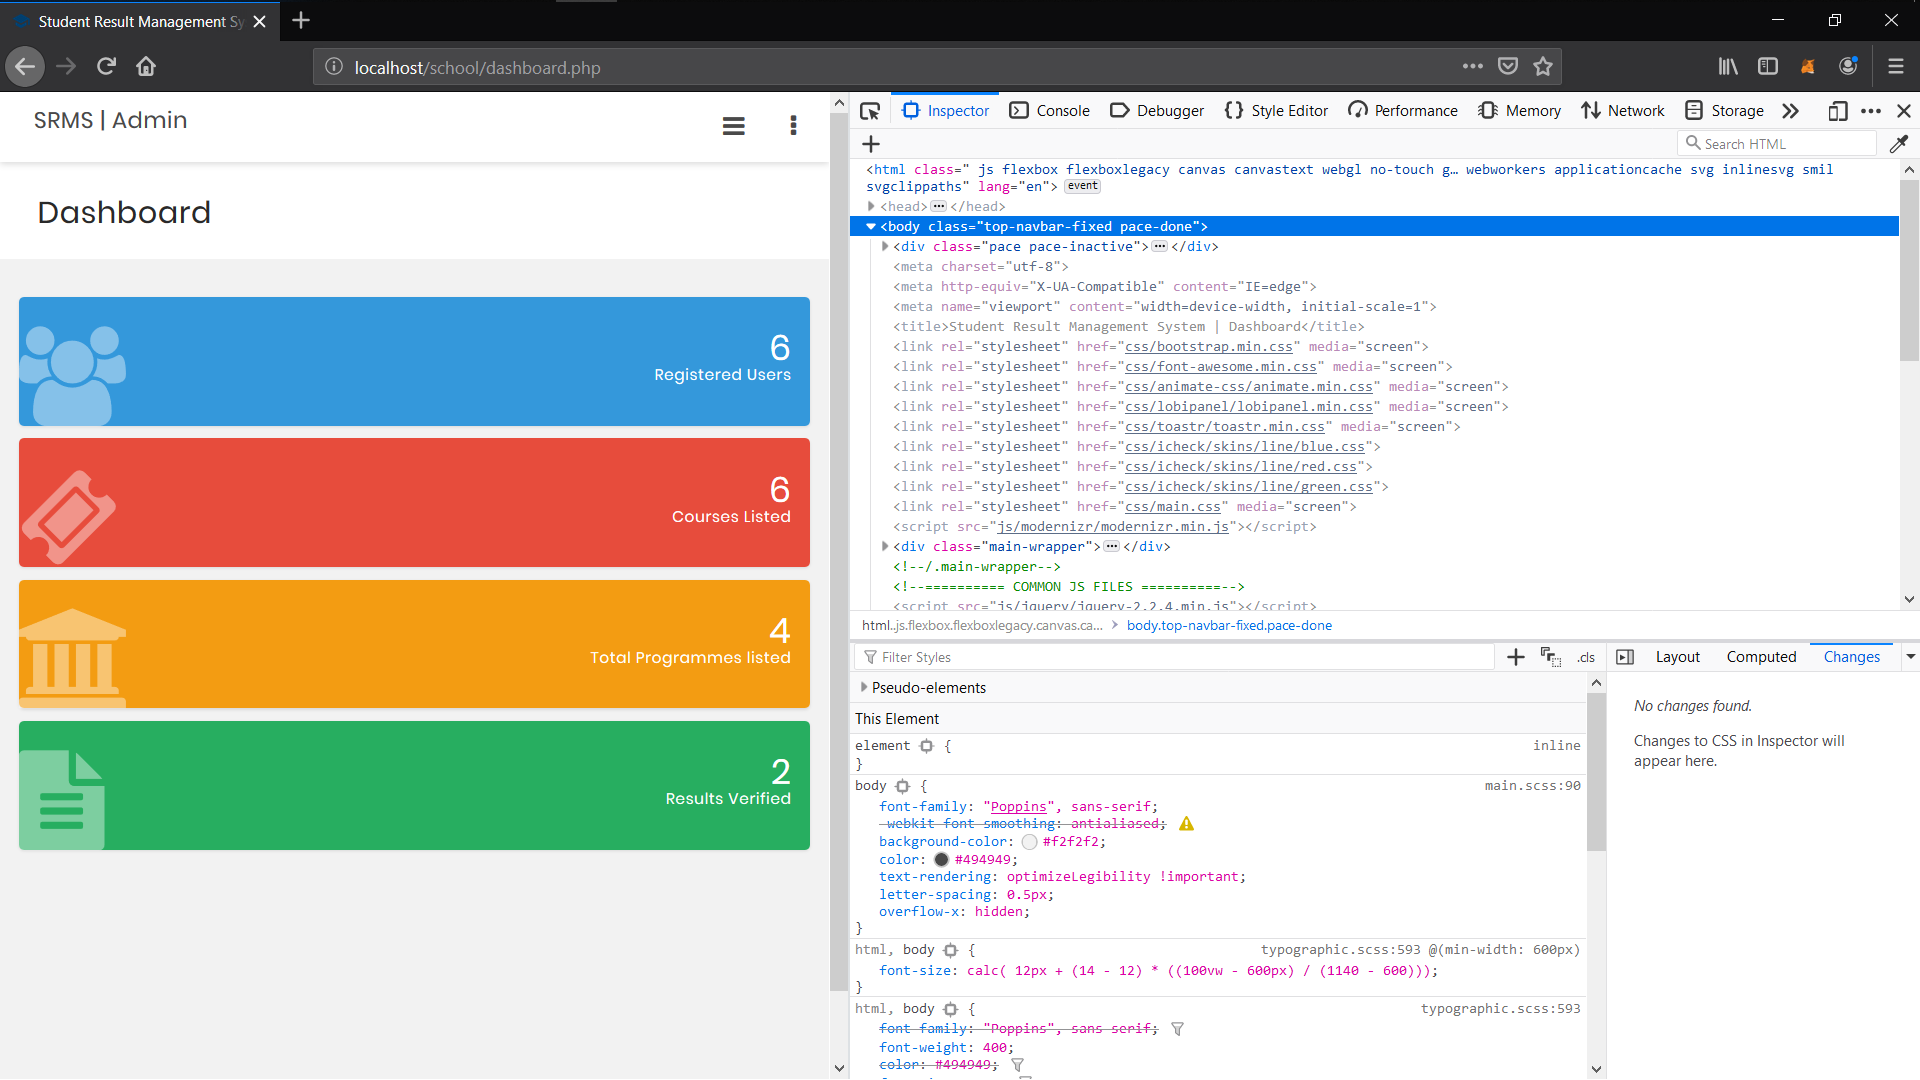
\includegraphics[scale=0.3]{images/dev_tools.png}
\caption{Developer tools opened in chrome to debug the Dashboard.}
\end{figure}

\begin{figure}[H]
\center
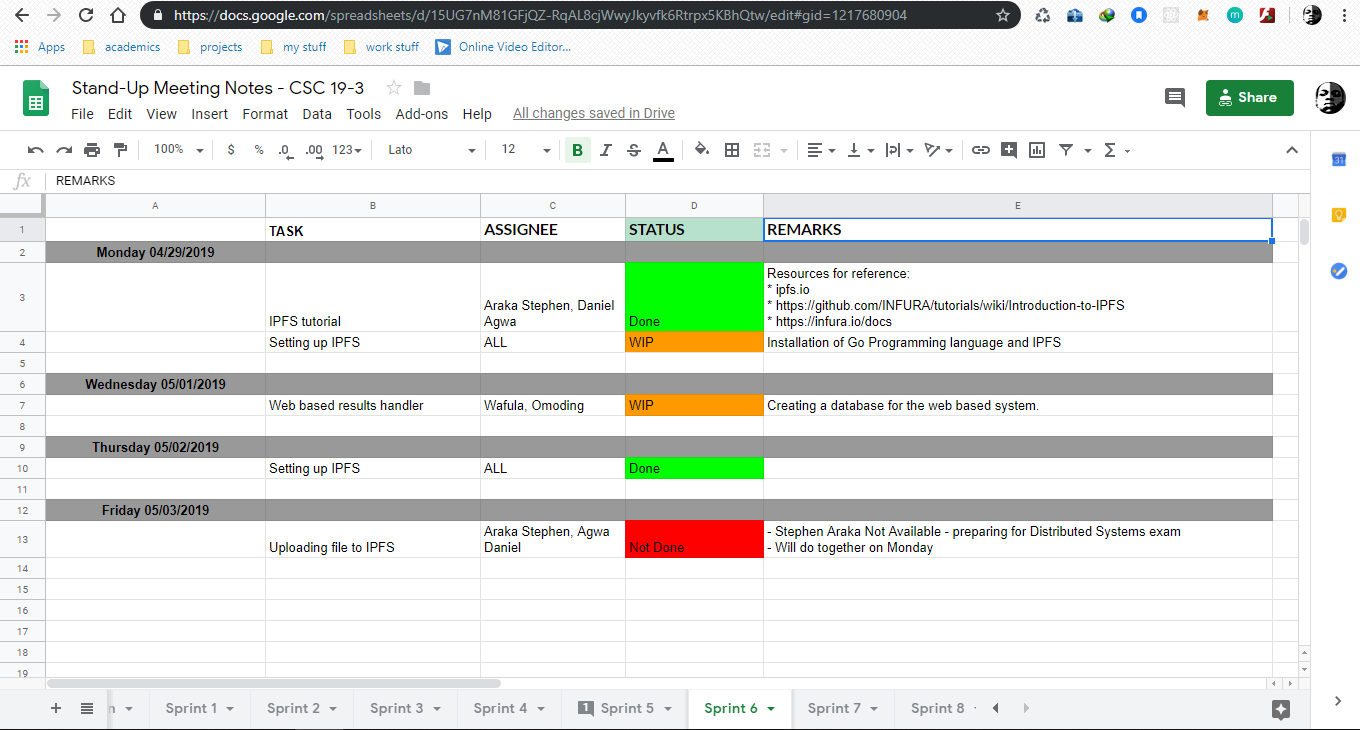
\includegraphics[scale=0.3]{images/docs.png}
\caption{Google document for Stand Up meetings and follow up}
\end{figure}

\begin{figure}[H]
\center
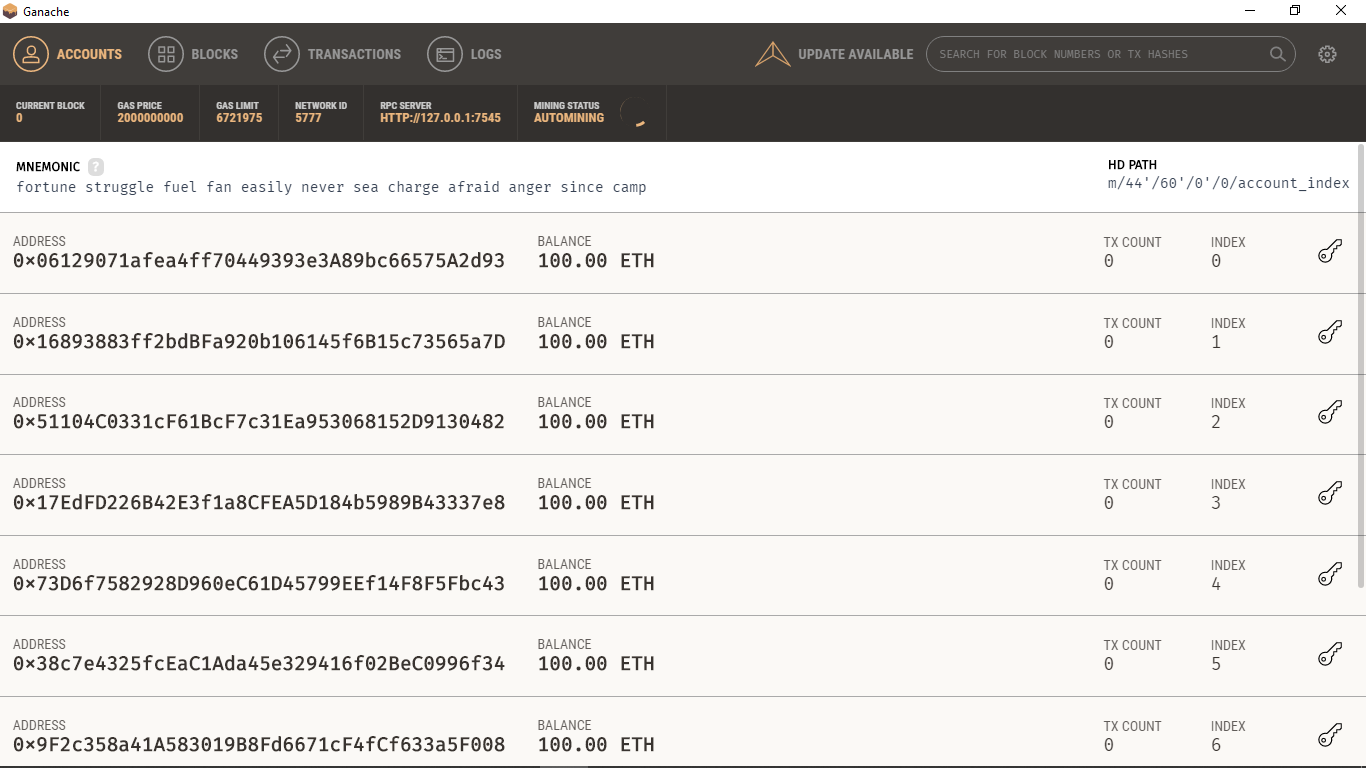
\includegraphics[scale=0.3]{images/ganache.png}
\caption{Accounts in Ganache: A local instance of the Ethereum blockchain}
\end{figure}

\section{Appendix B: Samples from the Implementation Process}

\begin{figure}[H]
\center
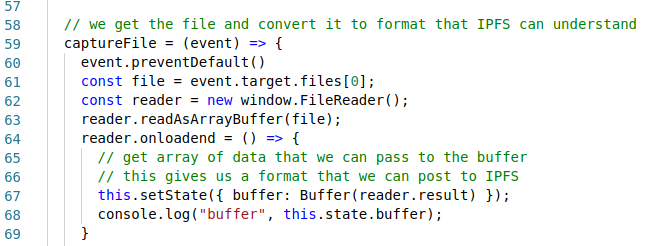
\includegraphics[scale=0.8]{images/codeconvert.png}
\caption{Conversion of file to an IPFS-valid format}
\end{figure}

\begin{figure}[H]
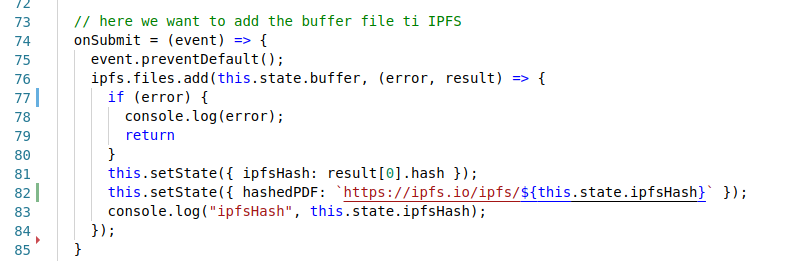
\includegraphics[scale=0.8]{images/codesubmit.png}
\caption{Conversion of file to an IPFS-valid format}
\end{figure}

\begin{figure}[H]
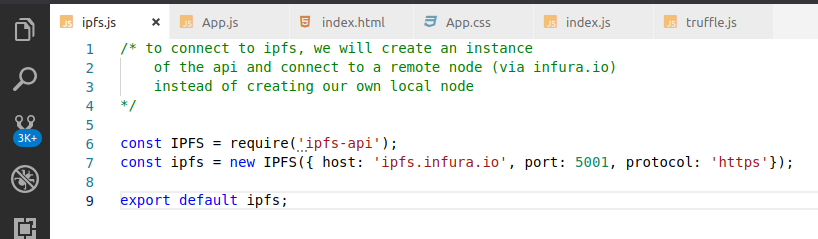
\includegraphics[scale=0.5]{images/codeinfura.png}
\caption{Accessing IPFs public node using the Infura API}
\end{figure}

\section{Appendix C: Images of the Application}
\begin{figure}[H]
\center
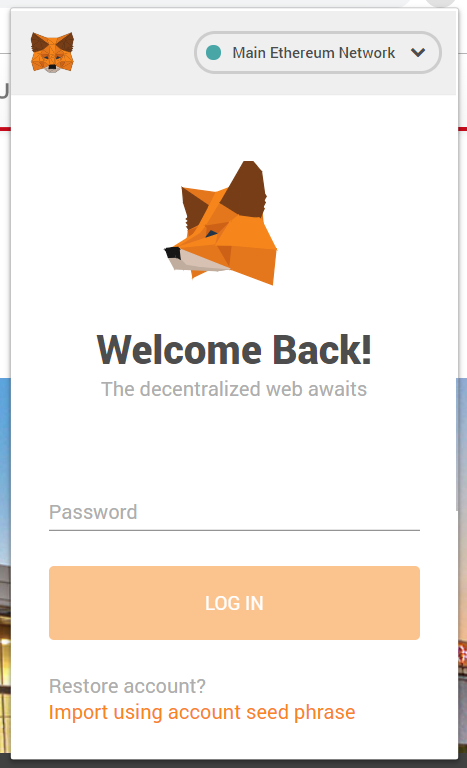
\includegraphics[scale=0.6]{images/metamasklogin.png}
\caption{Logging in to the ethereum network}
\end{figure}

\begin{figure}[H]
\center
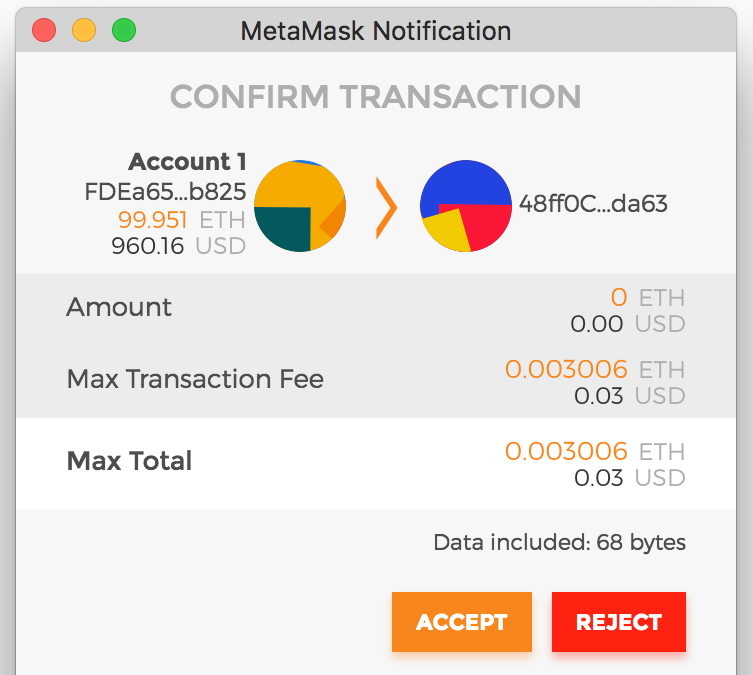
\includegraphics[scale=0.4]{images/MetamaskNotification.png}
\caption{A transaction awaiting confirmation from the user.}
\end{figure}